\chapter{Introduction}

\textbf{What is a plasma and why is it magnetically confined for nuclear fusion devices?}

A fusion plasma is a fully ionized gas whose behavior is dominated by long-range electric and magnetic fields. A major consequence of this behavior is that a plasma is an exceptionally good conductor of electricity, its conductivity implies that the plasma inside is shielded from DC electric fields $\bar{E}$ to a very large degree. On the other hand, DC magnetic fields $\bar{B}$ can penetrate and it is these fields that provide plasma confinement, hence the name "magnetic confinement" ~\cite[Chapter~6]{Freidberg2007}.\smallskip

\textbf{Why do we need magnetic fields in nuclear fusion devices ?}
\smallskip

Magnetic fields are needed to confine the hot plasma and keep it away from the machine walls.  In a generic magnetic fusion reactor the basic properties of magnetic fields require  a toroidal geometry so it can hold the plasma equilibrium ~\cite[Chapter~4]{Freidberg2007}. The properties of the magnetic fields require a toroidal geometry for confining magnetically the plasma. Trajectories of particles in the presence of magnetic fields are described by the Lorentz force equation $m \frac{d\bar{v}}{dt}=q(\bar{E}+\bar{v}\times \bar{B})$, which implies $\frac{d\bar{r}}{dt}=\bar{v}$, the combined perpendicular and parallel motion of a charged particle corresponds to a helical trajectory as  depicted in figure ~\ref{Helical}. If particles stream in a cylindrical device, they would collide with the wall due to the motion of the particles, a magnetic device whose lines wrapped around  a toroidal shape  prevent free streaming end loss, making obvious why the magnetic geometry for confining the plasma has to be toroidal.\smallskip

\begin{figure}
	\centering
	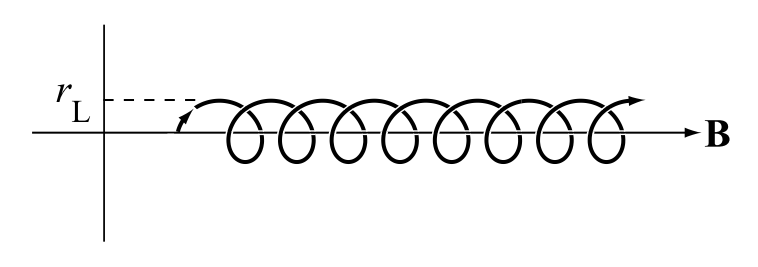
\includegraphics[width=0.525\textwidth]{Chp1/Helical_tray.png}
	\caption{  Helical trajectory of a charged particle in a uniform magnetic field ~\cite[Chapter~8]{Freidberg2007}.\label{Helical}}
\end{figure}

\section{Behind the plasma current}

Considering the drift of guiding center of a charged partice in a simple toroidal field in cylindrical coordinates $(R,\varphi,z)$. The component of the magnetic field $B_\varphi$ is the toroidal field and it decreases in the for of 1/R outward. The magnetic lines of force are circles around z axis. Particles in this  torus run fast in the toroidal direction and drift slowly in the z direction as shown in figure~\ref{TDrift}, this drift is called toroidal drift. As a consequence  using only a toroidal component of magnetic field is not sufficient for confining the plasma inside a toroidal device or a tokamak ~\cite[Chapter~3]{Miyamoto2011}.\smallskip


\begin{figure}
	\centering
	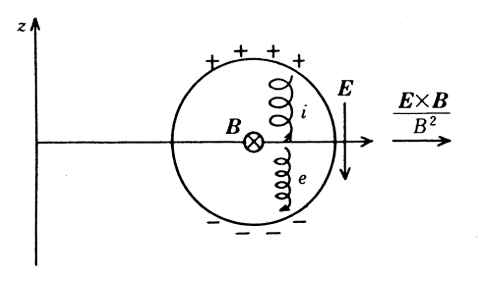
\includegraphics[width=0.55\textwidth]{Chp1/ToroidalDrift.png}
	\caption{Toroidal drift, particles drift in the vertical direction. ~\cite[Chapter~3]{Miyamoto2011} \label{TDrift}}
\end{figure}



All toroidal plasmas experience an outward toroidal force along $R$ direction, to establish toroidal force balance,  an inwardly pointing restoring force is required. One of the outwardly force generated by the toroidal configuration is called the "hoop force" and is analogous to  to the outward expansion force generated by the current flowing in a circular loop of wire. For a magnetic confined toroidal plasma this current correspondes to a toroidal current flowing in the plasma. If a current is induced in a toroidal plasma, the component of magnetic field around the magnetic axis (which is also called minor axis) is introduced. This component $B_P$ is called poloidal magnetic field and has components in $(R,z)$. \smallskip The poloidal field in a tokamak is mainly produced by the induced plasma toroidal current.  


$this is achieved by means of the application of an external vertical field.$




Typical operation of a tokamak discharge starts with the establishment of a large, steady, toroidal, magnetic field. Next, neutral gas is injected into the vacuum chamber and often pre-ionized. The transformer induced toroidal current or simply called plasma current $I_p$ is then ramped up to its maximum value and maintained for the “flat top” portion of the pulse~\cite[Chapter~13]{Freidberg2007}.

\section{Tokamak plasma control}

Tokamaks are basically devices with an axisymmetric configuration with a large toroidal magnetic field and a DC toroidal current, given its physical characteristics and its performance until now is presently the leading candidate to become the world’s first fusion reactor. During the start up and subsequent approximately steady state phase of many fusion plasma discharges a toroidal current is induced in the plasma by means of transformer action with the plasma being the secondary of the transformer  ~\cite[Chapter~9]{Freidberg2007}. Sometimes “poloidal field coils” means both the equilibrium field coils and the ohmic heating coils. By raising the current of the primary windings of the current transformer (ohmic heating coils), a current is induced in the plasma, which acts as the secondary winding. \smallskip

Control engineering for magnetic confined plasmas  embrace different types of techniques and they are use for the controlling different kind of variables and characteristics of the machine and the plasma.\smallskip  


\section{Thesis outline}

This work is divided in 5 chapters.

Chapter 2 explores the plasma control systems implemented in different tokamaks around the world and addresses some important theoretical concepts to be applied in the further chapters.\smallskip